\documentclass[a4paper,10pt]{article}
\usepackage[english]{babel}
\usepackage[utf8]{inputenc}
\usepackage{graphicx}
\usepackage{amsmath,amssymb}
\usepackage{hyperref, url}
\usepackage{listings}
\usepackage[multiple]{footmisc}
\usepackage[english]{babel}
\usepackage{float}
\parindent 0mm
\parskip 3mm

% add your name and student number in parenthesis
\title{ICS-E4020: Week 4 - Correlated pairs GPU}
\author{Néstor Castillo García (472081)\\ 
       {\tt nestor.castillogarcia@aalto.fi}}
\begin{document}

\maketitle

\section{Correlated pairs in GPU CP9 optimised}

\subsection{Description}

Using CUDA, an efficient working solution that solved the image correlation problem on the GPU was done.


\subsection{Hardware}
The computers had the following specifications: Intel Xeon E3-1230v2, 4 cores, 8 thread, 3,3 GHz, RAM: 16 GB, GPU: Nvidia K2000.

\subsection{Performance}
As the focus of this exercise in performance, it was heavily optimised. This GPU version did the correlated pairs task of a 4000 x 4000 image in less than 1s; 10 times faster than a eight-threaded. The focus of this approach was to maximise the number of arithmetic operation per memory transfer and also to used shared memory per block of threads because it is much more faster than the global memory. 



\begin{figure}[H]
\centering
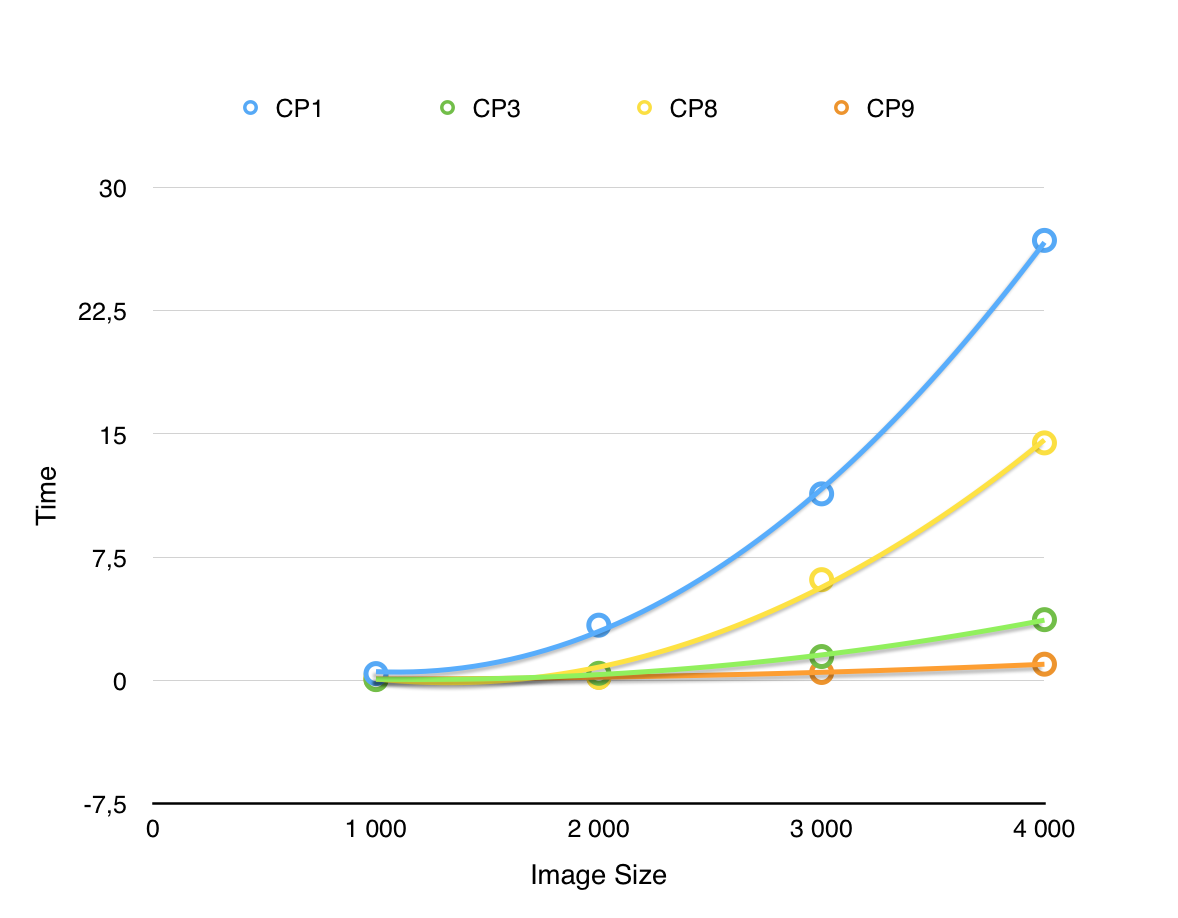
\includegraphics[width=1\textwidth]{figures/w5-comparison}
\caption{Scalability comparison between single threaded, multithreaded, multithreades vectorized and GPU implementations}
\label{fig:pca_type}
\end{figure}


The code was profiled with nvidia profiler and it was found that the kernel execution time occupies 97,5\% of the total time. Thus, the cudaMemCopy instructions occupy a small amount of time compared to the kernel execution. 

\begin{figure}[H]
\centering
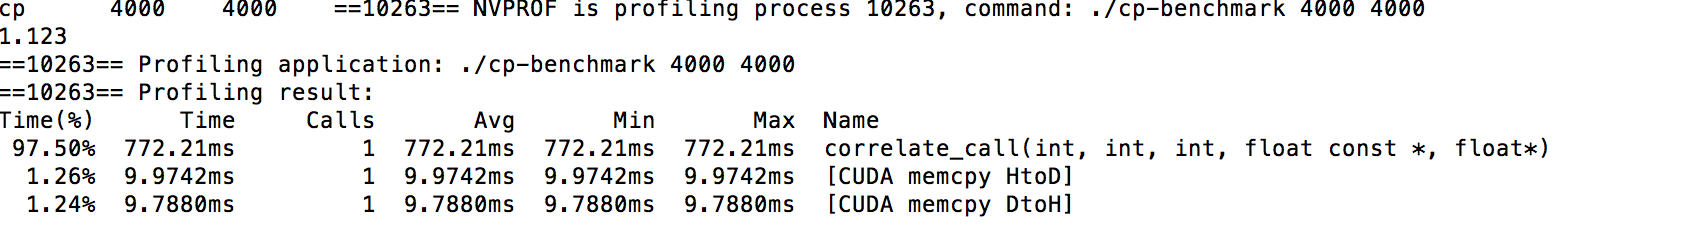
\includegraphics[width=1.3\textwidth]{figures/w5_timing}
\caption{Detailed execution time in a 4000 x 4000 image in comparison to cp8 in cp9 memcopy appears to be a little more relevant}
\label{fig:pca_type}
\end{figure}

\begin{figure}[H]
\centering
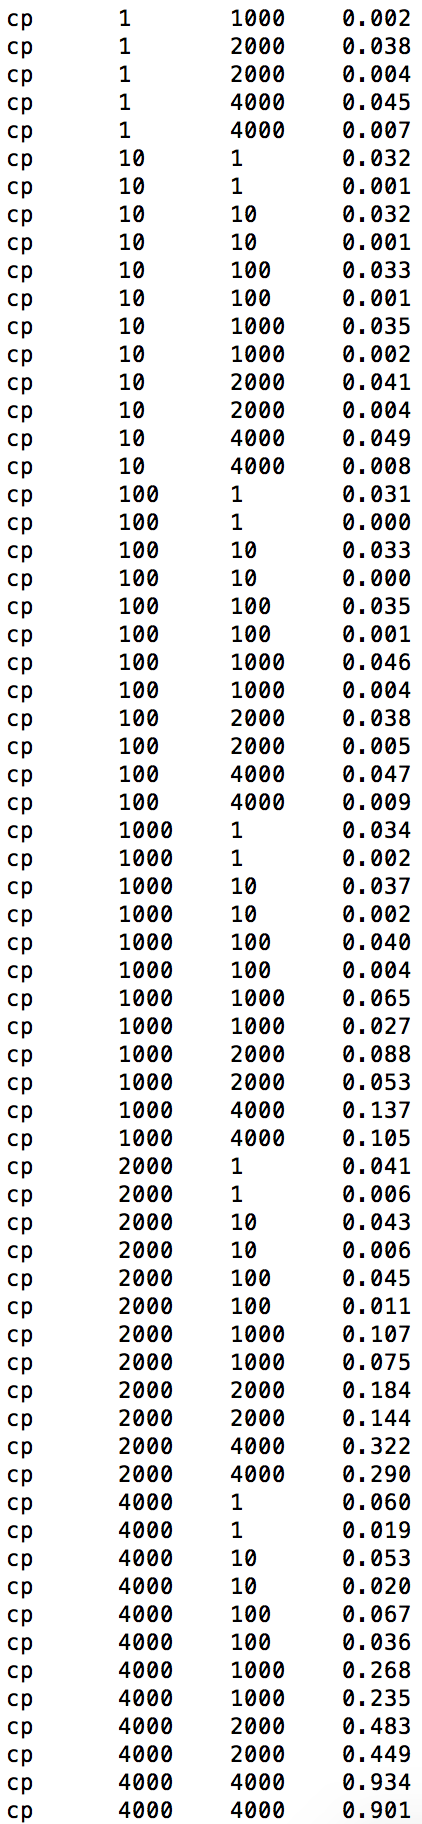
\includegraphics[width=0.3\textwidth]{figures/w5_benchmark}
\caption{Benchmark results}
\label{fig:pca_type}
\end{figure}




I\end{document}